\section{Profilo alare NACA 0015}
Nel presente esperimento sono valutate le caratteristiche aerodinamiche del profilo alare NACA 0015 mediante la misura della distribuzione di pressione al variare dell'incidenza e del numero di Reynolds. Sono inoltre determinate le curve del coefficiente di portanza $C_L(\alpha)$ e del coefficiente di momento aerodinamico $C_M(\alpha)$ rispetto all'incidenza $\alpha$ e la posizione del centro di pressione e del fuoco del profilo alare.
\begin{figure}[H]
    \centering
    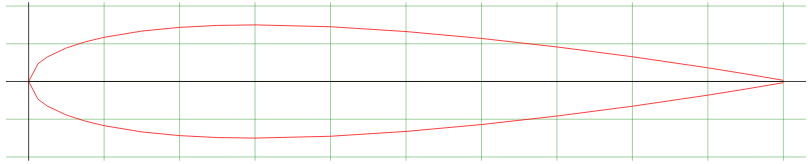
\includegraphics[width=\textwidth]{images/5/naca0015airfoiltools.png}
    \caption{Profilo alare NACA 0015}
\end{figure}

\subsection{Geometria del profilo alare}
I profili alari NACA sono forme geometriche standardizzate sviluppate dal National Advisory Committee for Aeronautics (NACA) degli Stati Uniti d'America. Un profilo alare NACA è definito da un numero, solitamente di quattro o cinque cifre, che ne determina le caratteristiche. In particolare, nei profili alari Naca a quattro cifre:
\begin{itemize}
    \item La prima cifra indica la curvatura massima come percentuale della corda;
    \item La seconda cifra fornisce la distanza del punto di massima curvatura dal bordo d'attacco espressa come percentuale della corda e in multipli di dieci;
    \item Le ultime due cifre descrivono il massimo spessore del profilo alare espresso come percentuale della corda.
\end{itemize}
Ad esempio, il profilo alare NACA 2412 presenta una curvatura massima del 2\%, situata al 40\% della corda partendo dal bordo d'attacco e ha uno spessore massimo del 12\% della corda. Nei profili alari NACA a quattro cifre lo spessore massimo è sempre posizionaot al 30\% della corda, sempre partendo dal bordo d'attacco.\\\\
Il profilo alare NACA 0015, preso in esame, è simmetrico, in quanto le cifre 00 indicano che non vi è una curvatura. Il 15 indica che lo spessore massimo è il 15\% della sua lunghezza.
\newpage
\noindent La formula per generare la forma di un profio alare NACA $00xx$, dove "$xx$" va sostituito con lo spessore massimo espresso come percentuale della corda, è:
\begin{equation*}
    y_t = 5tc\left[ 0.2969\sqrt{\frac{x}{c}} -0.1260\left(\frac{x}{c}\right) -0.3516\left(\frac xc \right)^2 + 0.2843 \left( \frac xc \right)^3 -0.1015 \left( \frac xc \right)^4 \right]
\end{equation*}
Dove:
\begin{itemize}
    \item $c$ è la lunghezza della corda;
    \item $x$ è la posizione lungo la corda da 0 a $c$;
    \item $y_t$ è metà dello spessore ad un dato valore di $x$;
    \item $t$ è lo spessore massimo espresso come frazione della corda, in modo che $100\,t$ sia uguale alle ultime due cifre del codice NACA.
\end{itemize}

\subsection{Descrizione dell'esperimento}
Nella presente attività, il profilo alare NACA 0015, di corda pari a $c=100$ mm, è studiato con l'utilizzo di una galleria del vento. Le forze di pressione esercitate dal fluido sul profilo giaccino sul piano del campo di moto. Le forza aerodinamica generata dal flusso può essere scomposta in due componenti, una parallela ed una normale alla velocità, rispettivamente la resistenza e la portanza. Tali forze risultano applicate in un punto detto centro di pressione.\\\\
Nota la distribuzione di pressione relativa $p-p_\infty$ sulla superficie del profilo $S$, la risultante delle forze aerodinamiche $F$ è data da:
\begin{equation*}
    F = \int_S (p-p_\infty)\vec n dS
\end{equation*}
Considerando un profilo immerso in una corrente uniforme di velocità $V_\infty$, posto ad incidenza $\alpha$, si utilizzano i pedici $+$ e $-$ per indicare le grandezze riferite rispettivamente a dorso e ventre del profilo.\\\\
Considerando un tratto di superficie del dorso di profondità unitaria, si ha:
\begin{equation*}
    dF_+ = (p_+ - p_\infty)(ds_+ \cdot 1)
\end{equation*}
La sua scomposizione lungo le coordinate $x$ e $y$, indicando con $\gamma$ l'angolo che rappresenta la pendenza locale della superficie del profilo, è:
\begin{equation*}
    dF_+|_x = (p_+ - p_\infty)(ds_+)\sin \gamma \quad dF_+|_y = (p_+ - p_\infty)(ds_+)\cos \gamma
\end{equation*}
Analogamente per il ventre:
\begin{equation*}
    dF_-|_x = (p_- - p_\infty)(ds_-)\sin \gamma \quad dF_-|_y = (p_- - p_\infty)(ds_-)\cos \gamma
\end{equation*}
Integrando tali forze elementari, si ricavano le componenti $R_x$ ed $R_y$ della forza aerodinamica risultante $F$:
\begin{equation*}
    R_x = \int_0^c (dF_+|_x + dF_-|_x)dx
\end{equation*}
\begin{equation*}
    R_y = \int_0^c (dF_+|_y + dF_-|_y)dy
\end{equation*}
Dalle due componenti si ricavano la portanza $L$ e la resistenza $D$ che risultano essere le componenti della forza aerodinamica proiettate rispettivamente perpendicolarmente e parallelamente alla velocità $V_\infty$ a monte del profilo:
\begin{equation*}
    L = R_y \cos \alpha + R_x \sin \alpha
\end{equation*}
\begin{equation*}
    D = R_x \cos \alpha + R_y \sin \alpha
\end{equation*}
Per piccoli angoli di incidenza, si può approssimare:
\begin{equation*}
    L\approx R_y = \int_0^c \left[ (p_--p_\infty) - (p_+-p_\infty) \right] dx
\end{equation*}
Definendo il coefficiente di pressione:
\begin{equation*}
    c_p = \frac{p-p_\infty}{\frac12 \rho V_\infty^2}
\end{equation*}
Si può riscrivere l'espressione della portanza come:
\begin{equation*}
    L = \frac12 \rho V^2_\infty \int_0^c (c_{p-}-c_{p+})dx
\end{equation*}
Introducendo il coefficiente portanza, e considerando un flusso bidimensionale, si può adimensionalizzare la portanza rispetto ad una superficie di larghezza pari alla corda $c$ e profondità unitaria:
\begin{equation*}
    c_L = \int_0^1(c_{p-}-c_{p+})d\left( \frac xc \right)
\end{equation*}
Il coefficiente di portanza è quindi valutato come l'area sottesa tra le curve $c_{p-}$ e $c_{p+}$.\\\\
Ulteriore obiettivo dell'attività consiste nel calcolo del coefficiente di momento $c_M$. Per comodità si sposta il punto di applicazione della portanza al bordo di attacco (leading edge) del profilo. Si assume per convenzione un momento positivo cabrante. Il momento elementare agente sull'elemento di superficie di profondità unitaria $ds$, trascurando il contributo dovuto al braccio lungo la direzione $y$, vale:
\begin{equation*}
    dM_{LE} = (dF_+|_y - dF_-|_y) x
\end{equation*}
Integrando si ottiene l'espressione per il momento al bordo di attacco:
\begin{equation*}
    M_{LE} = -\int_0^c \left[ (p_- - p_\infty)- (p_+ - p_\infty) \right] xdx
\end{equation*}
Con considerazioni analoghe alle precedenti si passa in termini adimensionali introducendo il coefficiente di momento:
\begin{equation*}
    c_{M_{LE}} = \frac{M_{LE}}{\frac12 \rho V_\infty^2 c^2} = -\int_0^1 (c_{p-}-c_{p+}) \left( \frac xc \right) d\left( \frac xc \right)
\end{equation*}
A questo punto, si può ricavare il centro di pressione $x_{cp}$. Conoscendo il momento al bordo di attacco e la portanza, si ha:
\begin{equation*}
    M_{LE} = -x_{cp} L
\end{equation*}
Che in termini adimensionali si traduce in:
\begin{equation*}
    c_{M_{LE}} = - \frac{x_{cp}}c c_L
\end{equation*}
Si ottiene quindi la relazione per la posizione del centro di pressione, che sarà funzione dell'incidenza:
\begin{equation*}
    \frac{x_{cp}}c = -\frac{c_{M_{LE}}}{c_L} = f(\alpha)
\end{equation*}
Dal coefficiente di portanza e dal coefficiente di momento al bordo di attacco è possibile stimare la posizione del fuoco, o centro aerodinamico $x_{ac}$, del profilo. Nel centro aerodinamico vale la proprietà focale: il momento aerodinamico rimane costante al variare dell'incidenza.\\\\
Il momento aerodinamico nel fuoco del profilo può essere scritto come:
\begin{equation*}
    M_{ac} = - L (x_{cp}-x{ac}) = -(Lx_{xp}) + Lx_{ac} = M_{LE} + Lx_{ac}
\end{equation*}
Tale relazione, in termini adimensionali, si traduce in:
\begin{equation*}
    c_{M_{ac}} = c_{M_{LE}} + c_L \frac{x_{ac}}c
\end{equation*}
Per il calcolo della posizione del fuoco è sufficiente quindi imporre la condizione focale:
\begin{equation*}
    \frac{\partial c_{M_{ac}}}{\partial \alpha} = 0
\end{equation*}
Avendo cura di sostituire l'espressione per il coefficiente di momento sul bordo di attacco e per il coefficiente di portanza nel tratto lineare delle rispettive curve.\\\\
Per un profilo in campo subsonico, la posizione del centro aerodinamico corrisponde a circa il 25\% della corda, mentre nel caso di campo supersonico il fuoco dei profili alare è posizionato in corrispondenza del 50\% della corda.\\\\
Una volta calcolato il fuoco del profilo è infine possibile ricavare il coefficiente di momento aerodinamico:
\begin{equation*}
    c_{M_{ac}} = c_{M_{LE}} + c_L \frac{x_{ac}}c
\end{equation*}
Per la proprietà focale, questo deve mantenersi costante al variare dell'incidenza.

\subsection{Catena di misura}
Per misurare la distribuzione di pressione sul dorso e sul ventre del profilo alare, questo è studiato in una galleria del vento aperta.
\begin{figure}[H]
    \centering
    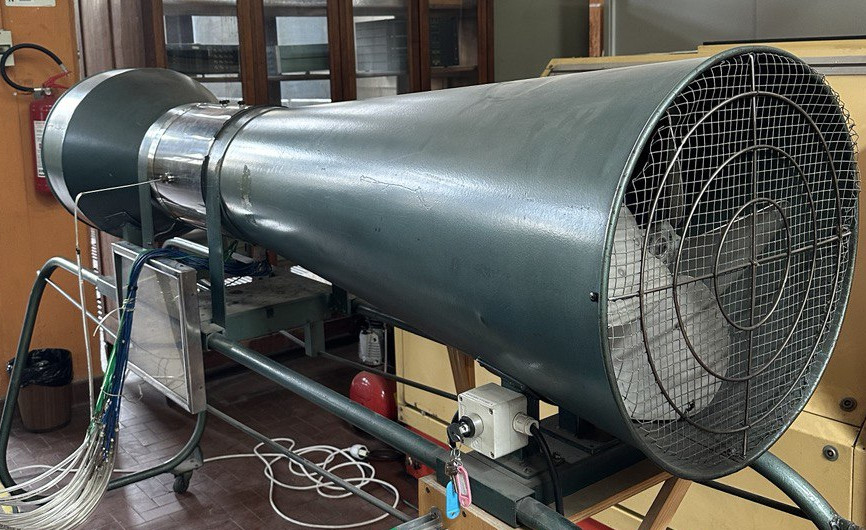
\includegraphics[width=.7\textwidth]{images/5/galleria.jpg}
    \caption{Galleria del vento}
\end{figure}

\noindent Per allineare il flusso e ridurre la turbolenza, all'entrata del convergente della galleria è presente un honeycomb.
\begin{figure}[H]
    \centering
    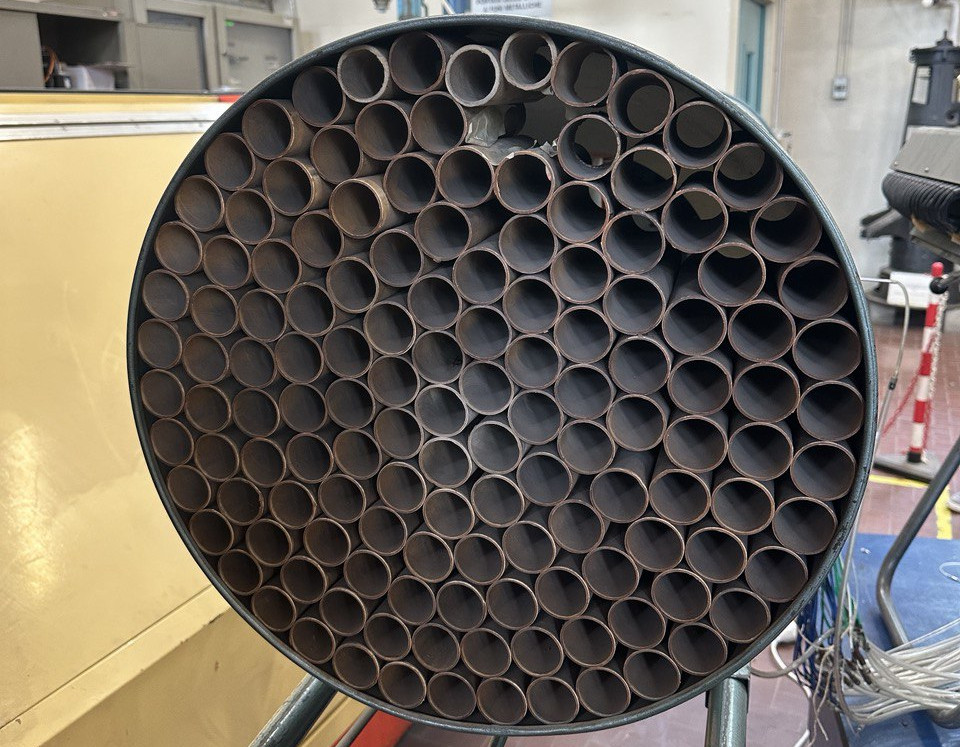
\includegraphics[width=.6\textwidth]{images/5/honeycomb.jpg}
    \caption{Honeycomb}
\end{figure}

\noindent Sul profilo alare sono posizionate 11 prese di pressione, alle seguenti coordinate dal bordo di attacco:
\begin{equation*}
    \left( \frac xc \right) = 0,\ 2.5,\ 5,\ 10,\ 20,\ 30,\ 40,\ 50,\ 60,\ 70,\ 80
\end{equation*}
Queste prese sono presenti solo su una faccia del profilo, questo perché data la geometria simmetrica, il campo di pressione rilevato sul dorso ad un angolo di incidenza positiva è uguale al campo di pressione che si rileva sul ventre allo stesso angolo di incidenza con segno opposto.
\begin{figure}[h]
    \centering
    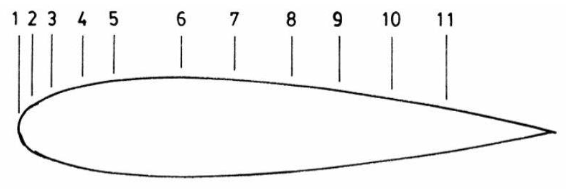
\includegraphics[width=.8\textwidth]{images/5/posizioneprese.png}
    \caption{Posizione delle prese statiche di pressione sul profilo alare}
\end{figure}

\noindent La misurazione della pressione statica localmente sul profilo è basata su una considerazione fondamentale, osservando le equazioni di Navier-Stokes specializzate per lo strato limite bidimensionale.
\begin{equation*}
    \begin{dcases}
        &\frac{\partial u}{\partial x} + \frac{\partial v}{\partial y} = 0\\
        & u\frac{\partial u}{\partial x} + v\frac{\partial u}{\partial y} = -\frac1\rho \frac{\partial P}{\partial x} + \nu\left( \frac{\partial^2 u}{\partial x^2} + \frac{\partial^2 u}{\partial y^2} \right)\\
        & u\frac{\partial v}{\partial x} + v\frac{\partial v}{\partial y} = -\frac1\rho \frac{\partial P}{\partial y} + \nu\left( \frac{\partial^2 v}{\partial x^2} + \frac{\partial^2 v}{\partial y^2} \right)
    \end{dcases}
\end{equation*}
Tenuto conto che nello strato limite tutte le grandezze variano rapidamente con l'ordinata $y$ e lentamente con l'ascissa $x$ e che è sempre verificata la condizione di piccole perturbazioni, la terza equazione si riduce a:
\begin{equation*}
    \frac{\partial P}{\partial y} = 0
\end{equation*}
Cioè la pressione statica nello strato limite lungo la coordinata $y$ rimane costante. Grazie a questa considerazione è possibile considerare la pressione statica misurata a parete uguale alla pressione statica appena fuori dallo strato limite, ottenendo quindi informazioni sul campo di moto attorno al profilo.\\\\
Oltre alle 11 prese di pressione statica sul profilo, sono presenti altre due prese subito a valle del convergente, una per la pressione totale ed una per la pressione statica. Queste 13 prese sono collegate tramite condotti pneumatici ad un multimanometro differenziale.\\\\
In particolare, la presa di pressione statica all'ingresso della camera di prova e la presa di pressione totale della corrente sono connesse con le canne 1 e 2 del multimanometro, le canne 3 e 4 sono libere e quindi rilevano la pressione ambiente mentre le altre 11 canne sono impegnate dai segnali delle prese su una delle due facce del profilo alare.
\begin{figure}[H]
    \centering
    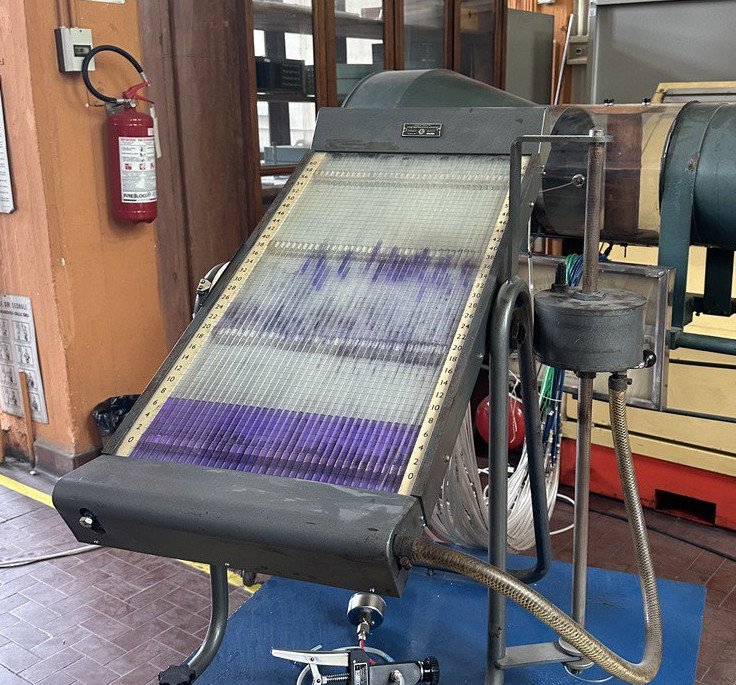
\includegraphics[width=.8\textwidth]{images/5/multimanometro.jpg}
    \caption{Multimanometro}
\end{figure}

\noindent Le canne manometriche sono inclinate con un angolo $\beta=15^\circ$ e riempite con alcool etilico, di densità nota $\rho_{fm} = 0.789$ g/cm$^3$.\\\\
Il peso specifico del fluido manometrico si ottiene come:
\begin{equation*}
    \gamma_{fm} = g_0 \rho_{fm} = 7732\ \text{N/m}^3
\end{equation*}
Inoltre, a partire dai valori di pressione e temperatura ambiente, si ricava la densità dell'aria dalla legge dei gas perfetti e la viscosità dinamica dalla legge di Sutherland:
\begin{equation*}
    \rho = \frac{p_{amb}}{RT_{amb}} \qquad \mu = 1.46\cdot10^{-6} \frac{T_{amb}^{3/2}}{T_{amb}+110}
\end{equation*}
Dalla legge di Stevino, misurando le altezze delle canne manometriche con l'apposita scala graduata in centimetri, si ricavano i valori di pressione:
\begin{equation*}
    (p-p_{ref}) = (h_{ref}-h) \gamma_{fm} \sin \beta
\end{equation*}
Dalla relazione di Bernoulli, si ottiene il valore della velocità indisturbata a monte:
\begin{equation*}
    V_\infty = \sqrt{\frac{2q}\rho} = \sqrt{\frac{2(p_{0\infty}-p_\infty)}{\rho}}
\end{equation*}
Pertanto si può valutare il coefficiente di pressione come:
\begin{equation*}
    c_p = \frac{p-p_{\infty}}{\frac12 \rho V_\infty^2} = \frac{p-p_\infty}{p_{0\infty}-p_\infty} = \frac{h_\infty-h}{h_\infty-h_{0\infty}}
\end{equation*}

\subsection{Procedura sperimentale}
L'esperimento è condotto variando l'angolo d'incidenza del profilo alare ruotandolo sul cinematismo e controllando i gradi di rotazione con un goniometro.\\\\
Ogni squadra ha utilizzato un diverso valore di portata, quindi un diverso numero di Reynolds, costante per tutte le incidenze esaminate.\\\\
Per ogni angolo di incidenza, si avvia la galleria, si attende il termine di eventuali fenomeni transitori e una volta che le canne manometriche si stabilizzano si registrano i rispettivi valori con una fotografia.\\\\
Si prendono prima tutti i dati ad angoli di incidenza positivi, rappresentativi dei profili di pressione sul dorso, poi si prendono le misure utilizzando gli stessi angoli di incidenza ma di segno negativo, rappresentativi dei profili di pressione sul ventre del profilo.\\\\
I dati grezzi ottenuti sono quindi manualmente riportati in una tabella ad esempio in Microsoft Excel. Le tabelle di dati grezzi ottenute per le quattro squadre per la presente attività sono riportate in appendice \ref{a5}.\\\\
Si riportano a seguire alcuni istogrammi rappresentativi delle colonne di fluido manometrico:
\begin{figure}[H]
    \centering
    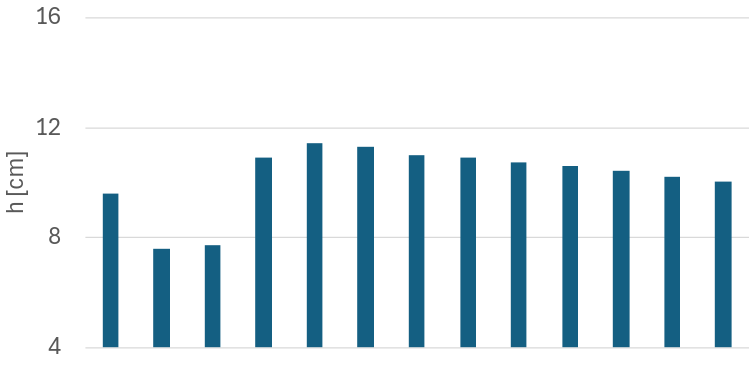
\includegraphics[width=.49\textwidth]{images/5/dsq1a0.png}
    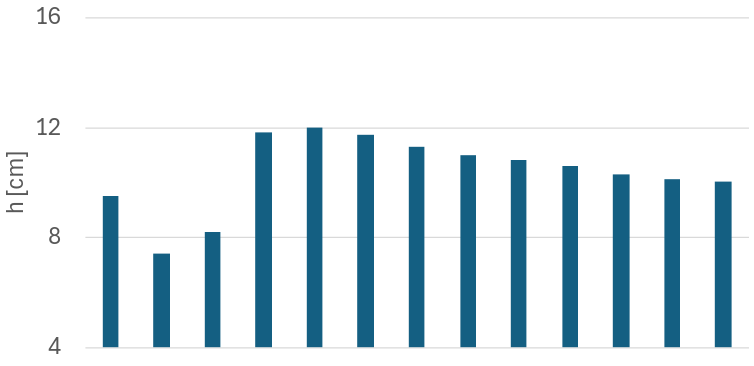
\includegraphics[width=.49\textwidth]{images/5/dsq1a2.png}
    \caption{Istogrammi per la squadra 1 ad incidenza 0 e 2 gradi}
\end{figure}

\begin{figure}[H]
    \centering
    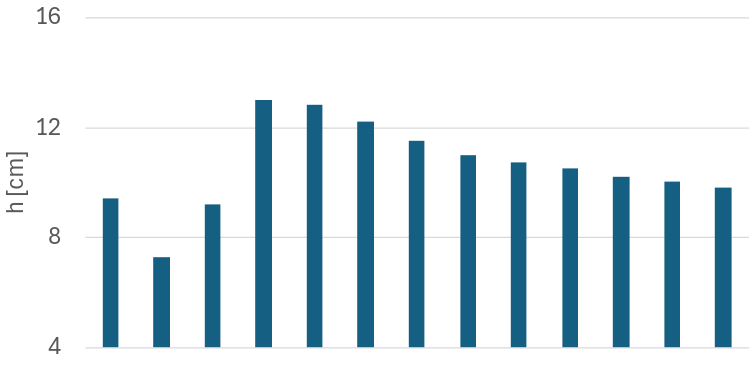
\includegraphics[width=.49\textwidth]{images/5/dsq1a4.png}
    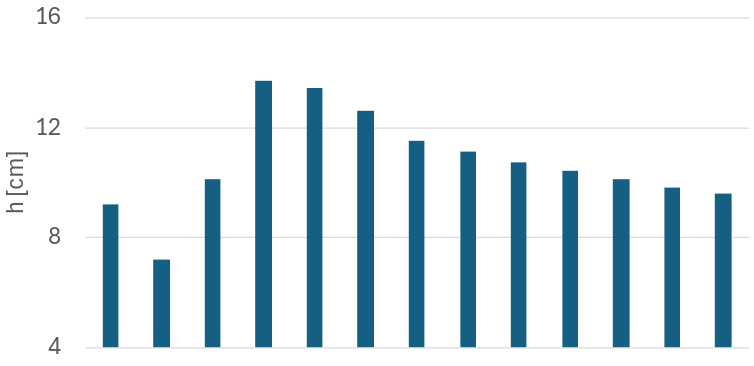
\includegraphics[width=.49\textwidth]{images/5/dsq1a6.png}
    \caption{Istogrammi per la squadra 1 ad incidenza 4 e 6 gradi}
\end{figure}

\begin{figure}[H]
    \centering
    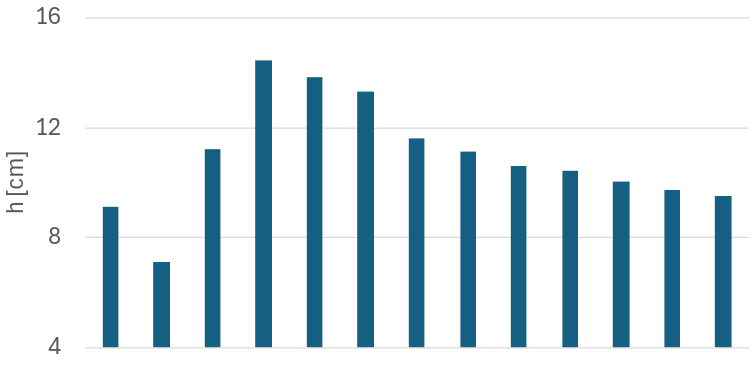
\includegraphics[width=.49\textwidth]{images/5/dsq1a8.png}
    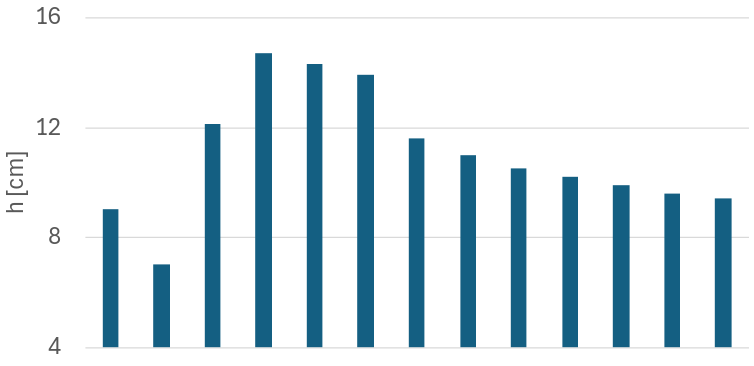
\includegraphics[width=.49\textwidth]{images/5/dsq1a10.png}
    \caption{Istogrammi per la squadra 1 ad incidenza 8 e 10 gradi}
\end{figure}

\begin{figure}[H]
    \centering
    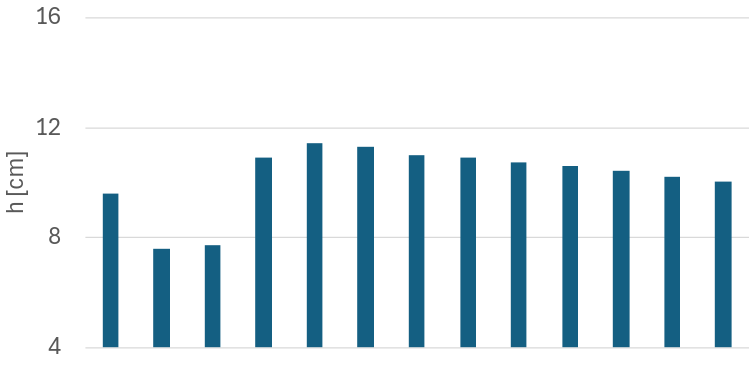
\includegraphics[width=.49\textwidth]{images/5/dsq1a0.png}
    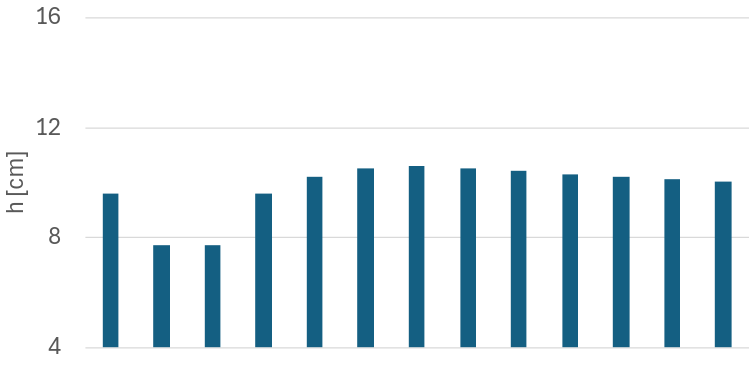
\includegraphics[width=.49\textwidth]{images/5/dsq1a-2.png}
    \caption{Istogrammi per la squadra 1 ad incidenza 0 e -2 gradi}
\end{figure}

\begin{figure}[H]
    \centering
    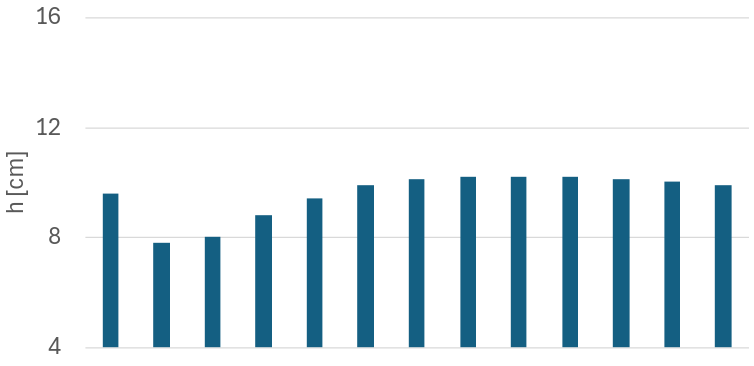
\includegraphics[width=.49\textwidth]{images/5/dsq1a-4.png}
    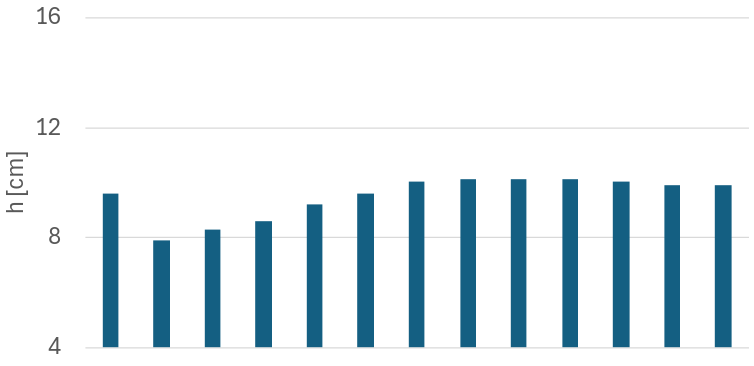
\includegraphics[width=.49\textwidth]{images/5/dsq1a-6.png}
    \caption{Istogrammi per la squadra 1 ad incidenza -4 e -6 gradi}
\end{figure}

\begin{figure}[H]
    \centering
    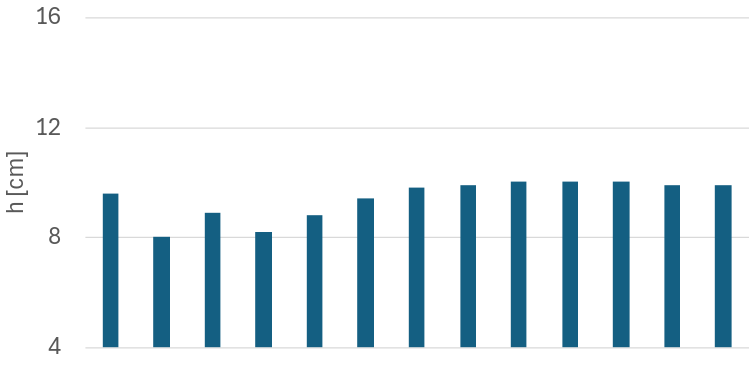
\includegraphics[width=.49\textwidth]{images/5/dsq1a-8.png}
    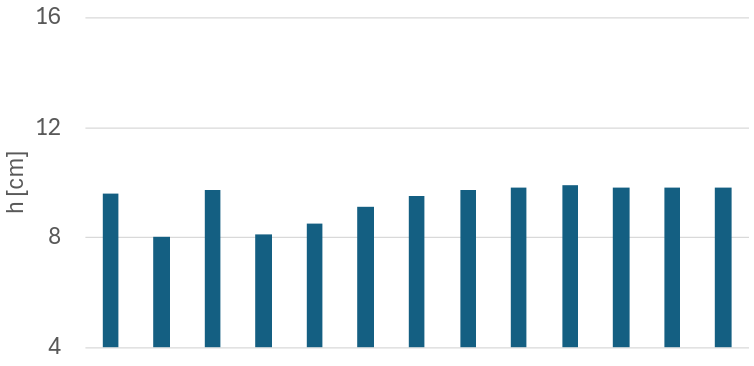
\includegraphics[width=.49\textwidth]{images/5/dsq1a-10.png}
    \caption{Istogrammi per la squadra 1 ad incidenza -8 e -10 gradi}
\end{figure}

\begin{figure}[H]
    \centering
    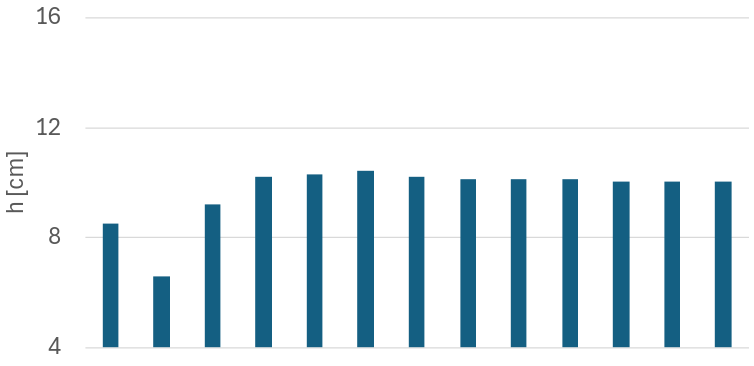
\includegraphics[width=.49\textwidth]{images/5/dsq1a14.png}
    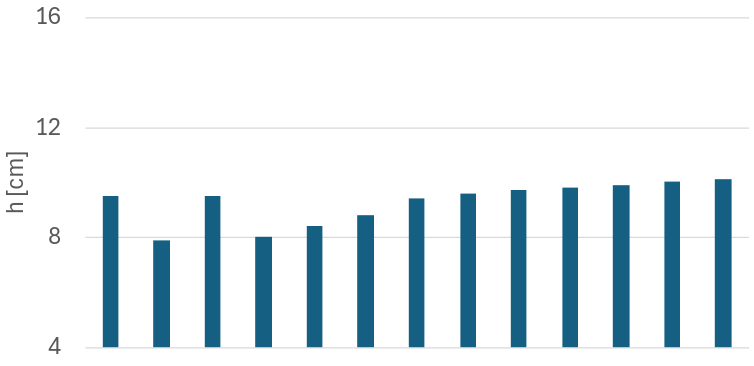
\includegraphics[width=.49\textwidth]{images/5/dsq1a-14.png}
    \caption{Istogrammi per la squadra 1 ad incidenza 14 e -14 gradi}
\end{figure}

\begin{figure}[H]
    \centering
    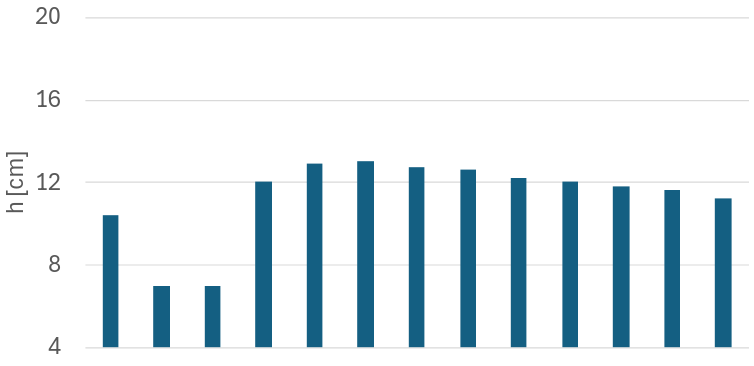
\includegraphics[width=.49\textwidth]{images/5/dsq2a0.png}
    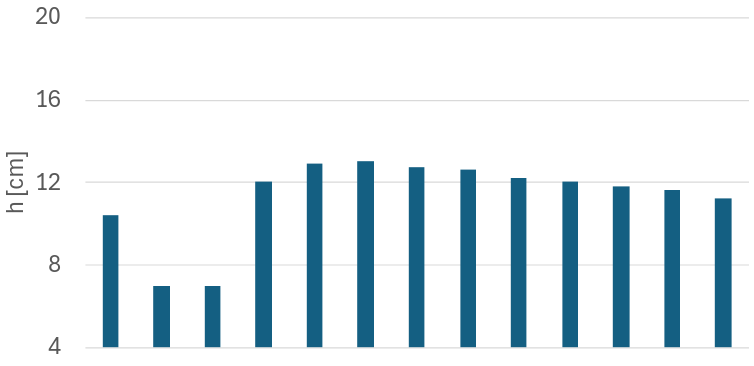
\includegraphics[width=.49\textwidth]{images/5/dsq2a2.png}
    \caption{Istogrammi per la squadra 2 ad incidenza 0 e 2 gradi}
\end{figure}

\begin{figure}[H]
    \centering
    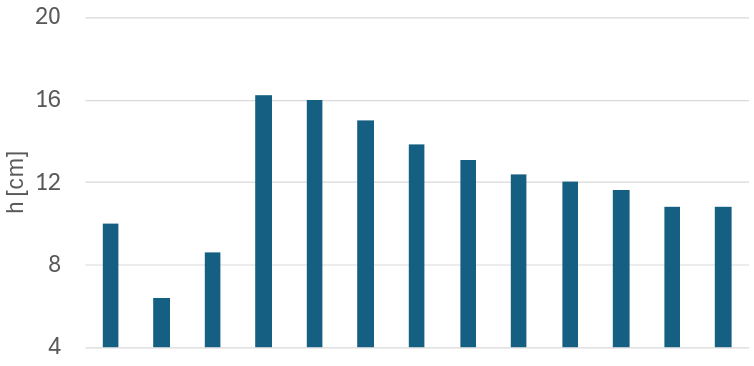
\includegraphics[width=.49\textwidth]{images/5/dsq2a4.png}
    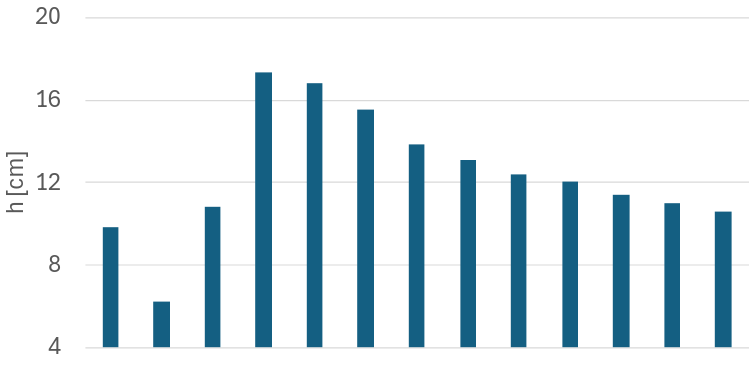
\includegraphics[width=.49\textwidth]{images/5/dsq2a6.png}
    \caption{Istogrammi per la squadra 2 ad incidenza 4 e 6 gradi}
\end{figure}

\begin{figure}[H]
    \centering
    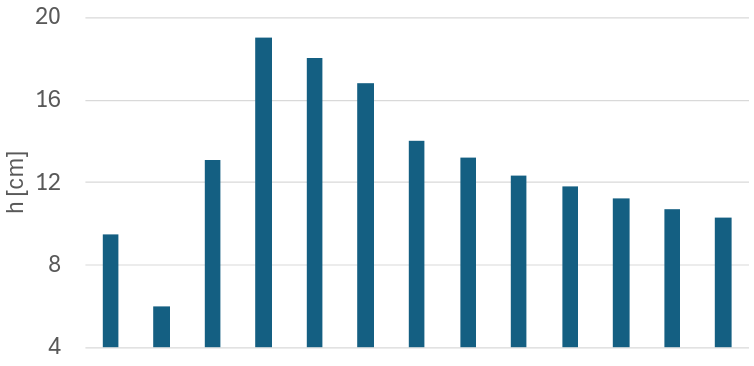
\includegraphics[width=.49\textwidth]{images/5/dsq2a8.png}
    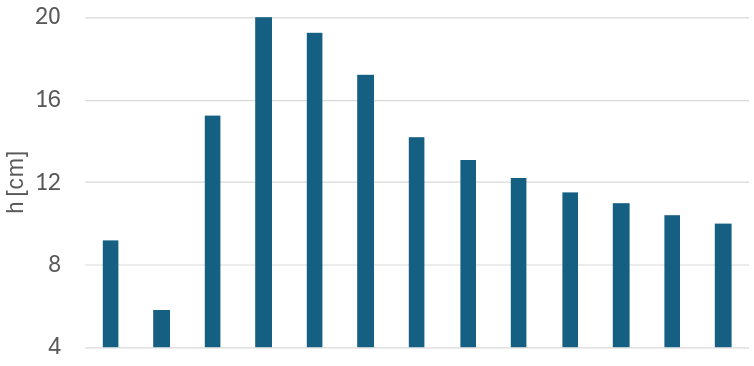
\includegraphics[width=.49\textwidth]{images/5/dsq2a10.png}
    \caption{Istogrammi per la squadra 2 ad incidenza 8 e 10 gradi}
\end{figure}

\begin{figure}[H]
    \centering
    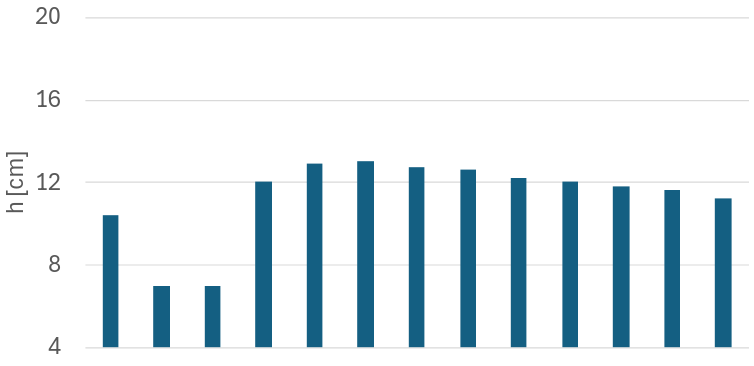
\includegraphics[width=.49\textwidth]{images/5/dsq2a0.png}
    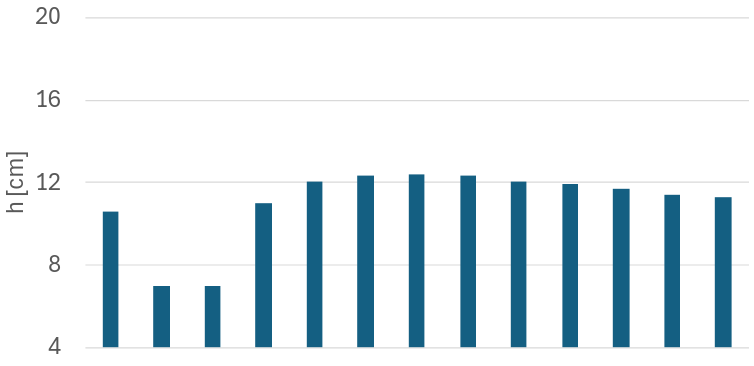
\includegraphics[width=.49\textwidth]{images/5/dsq2a-2.png}
    \caption{Istogrammi per la squadra 2 ad incidenza 0 e -2 gradi}
\end{figure}

\begin{figure}[H]
    \centering
    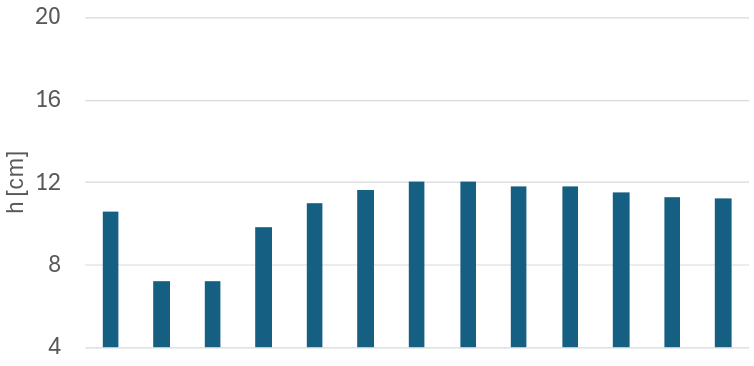
\includegraphics[width=.49\textwidth]{images/5/dsq2a-4.png}
    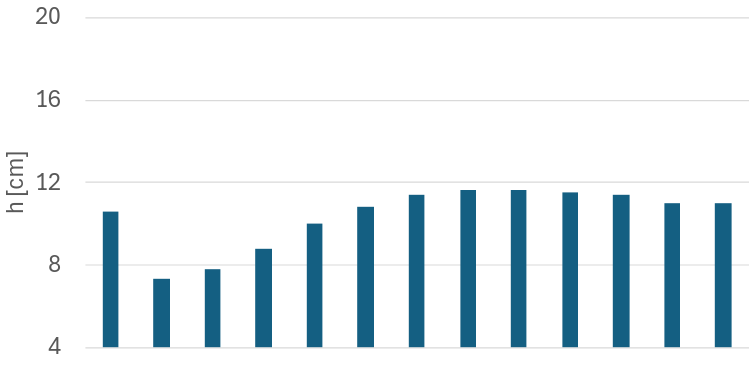
\includegraphics[width=.49\textwidth]{images/5/dsq2a-6.png}
    \caption{Istogrammi per la squadra 2 ad incidenza -4 e -6 gradi}
\end{figure}

\begin{figure}[H]
    \centering
    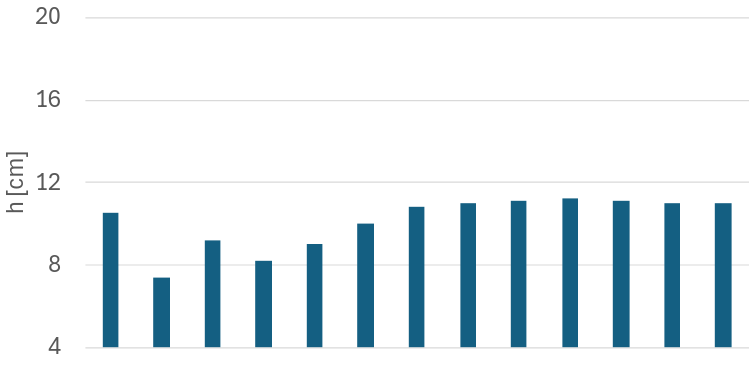
\includegraphics[width=.49\textwidth]{images/5/dsq2a-8.png}
    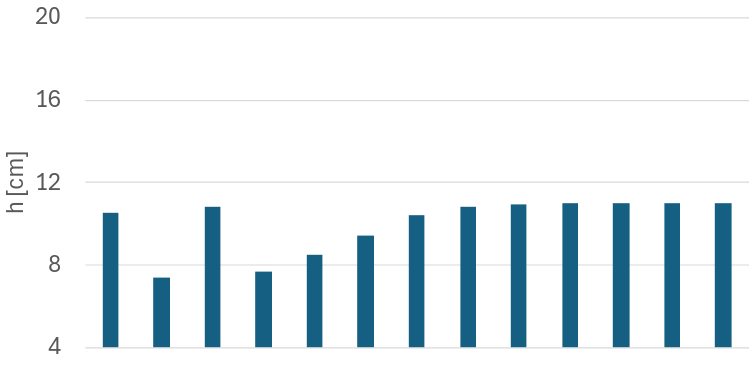
\includegraphics[width=.49\textwidth]{images/5/dsq2a-10.png}
    \caption{Istogrammi per la squadra 2 ad incidenza -8 e -10 gradi}
\end{figure}

\subsection{Analisi dati}
L'analisi dati per la presente attività è condotta con l'ausilio di un codice Python, riportato in appendice \ref{b5}.\\\\
Come prima operazione si calcola la densità e la viscosità dinamica, a partire dalla pressione e dalla temperatura ambiente, utilizzando la legge dei gas perfetti e la legge di Sutherland:
\begin{equation*}
    \rho = \frac{p_{amb}}{RT_{amb}} \qquad \mu = 1.46\cdot10^{-6} \frac{T_{amb}^{3/2}}{T_{amb}+110}
\end{equation*}
Poi, dalla relazione di Bernoulli, si ricava la velocità a monte per ogni misura:
\begin{equation*}
    V_\infty = \sqrt{\frac{2(h_{\infty}-h) \gamma_{fm} \sin \beta}{\rho}}
\end{equation*}
Quindi a seguire il numero di Reynolds:
\begin{equation*}
    Re = \frac{\rho V_\infty c}{\mu}
\end{equation*}
Si ottengono i seguenti numeri di Reynolds per le quattro squadre:
\begin{equation*}
    Re = 75000,\ 100000,\ 90000,\ 120000
\end{equation*}

\subsubsection{Coefficiente di pressione}
Dai dati sulle altezze delle canne manometriche è immediato ricavare i coefficienti di pressioni valutati ad ogni posizione sul profilo e per ogni incidenza:
\begin{equation*}
    c_p(x,\alpha) = \frac{h_\infty-h}{h_\infty - h_{0\infty}}
\end{equation*}
Per effettuare i seguenti calcoli è stata utilizzato un foglio di calcolo in Microsoft Excel. Dal valore del coefficiente di pressione è inoltre possibile ricavare i profili di velocità:
\begin{equation*}
    \frac{V(x,\alpha)}{V_\infty} = \sqrt{1-c_p}
\end{equation*}
Poiché, per motivi strutturali, non sono presenti prese di pressione statiche fino al bordo di fuga del profilo, bensì solo fino all'80\% della corda, è opportuno valutare il valore di coefficiente di pressione sul bordo di fuga interpolando i dati delle prese di pressione statica precedenti, con l'accortezza di rispettare la condizione di Kutta, tale per cui sul bordo di fuga:
\begin{equation*}
    p_+ = p_-
\end{equation*}
Utilizzando i coefficienti di pressione calcolati ed i coefficienti di pressione al bordo di attacco estrapolati, si ottengono i diagrammi riportati a seguire.
\begin{figure}[H]
    \centering
    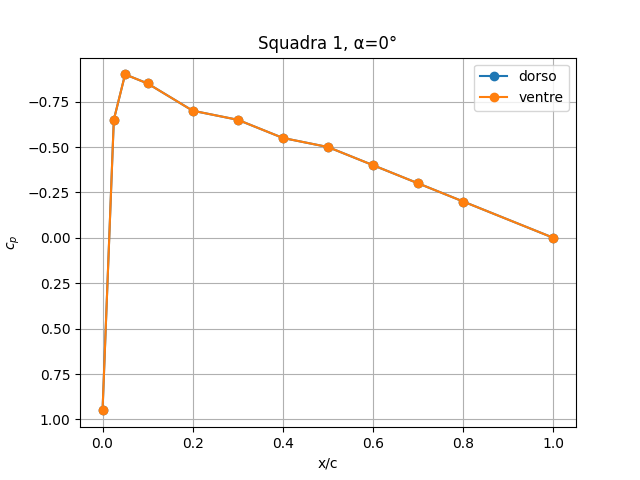
\includegraphics[width=.49\textwidth]{images/5/cp1 a=0.png}
    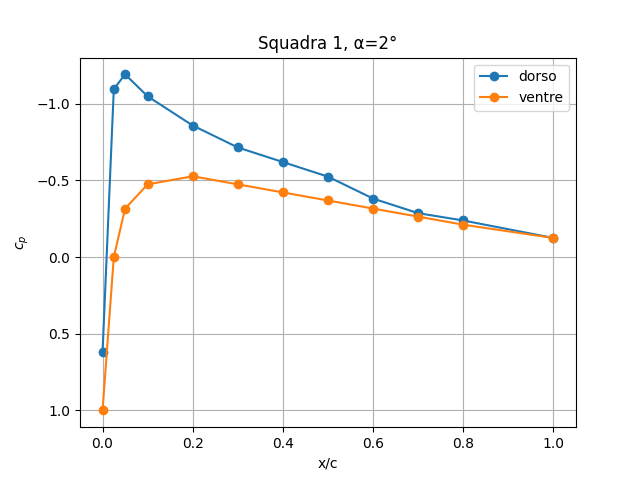
\includegraphics[width=.49\textwidth]{images/5/cp1 a=2.png}
    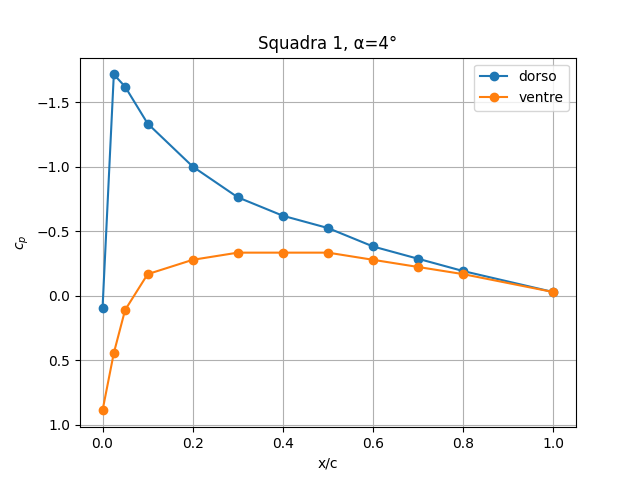
\includegraphics[width=.49\textwidth]{images/5/cp1 a=4.png}
    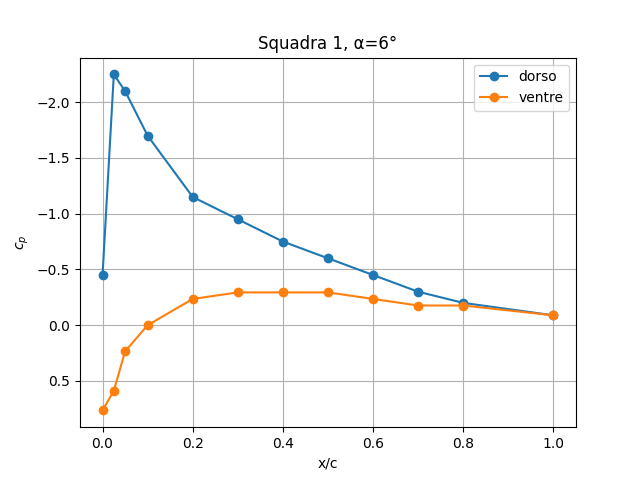
\includegraphics[width=.49\textwidth]{images/5/cp1 a=6.png}
    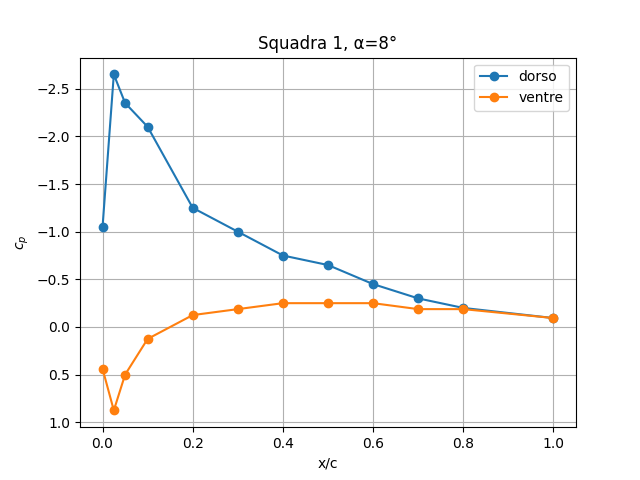
\includegraphics[width=.49\textwidth]{images/5/cp1 a=8.png}
    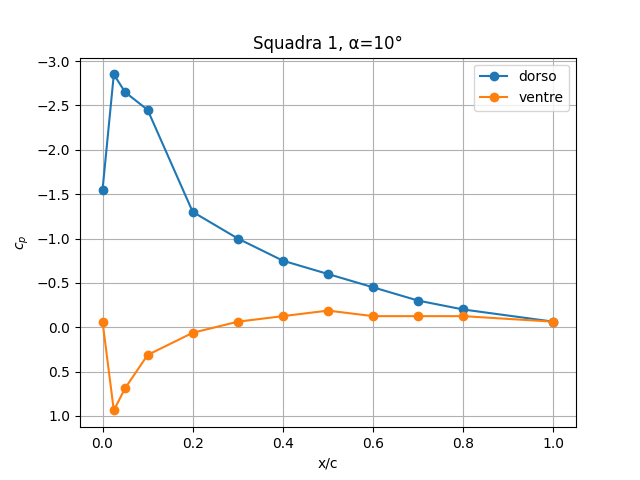
\includegraphics[width=.49\textwidth]{images/5/cp1 a=10.png}
    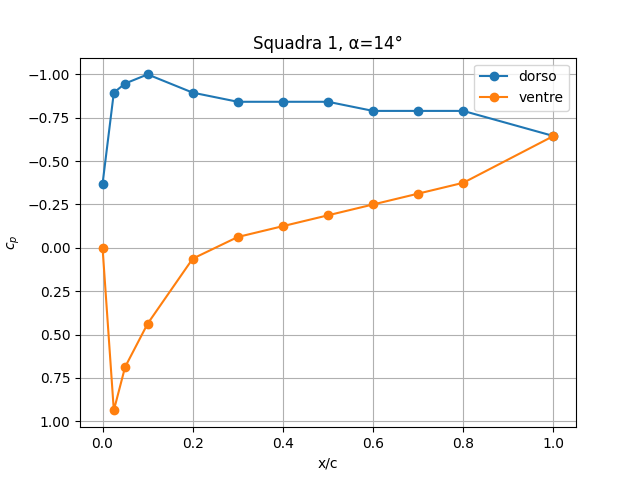
\includegraphics[width=.49\textwidth]{images/5/cp1 a=14.png}
    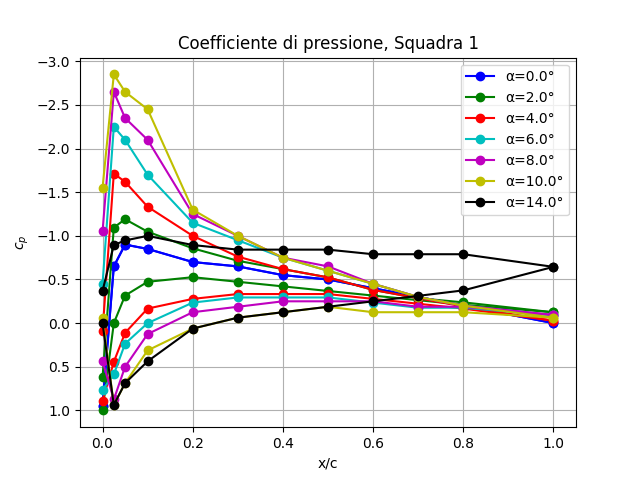
\includegraphics[width=.49\textwidth]{images/5/cp1.png}
\end{figure}
\begin{figure}[H]
    \centering
    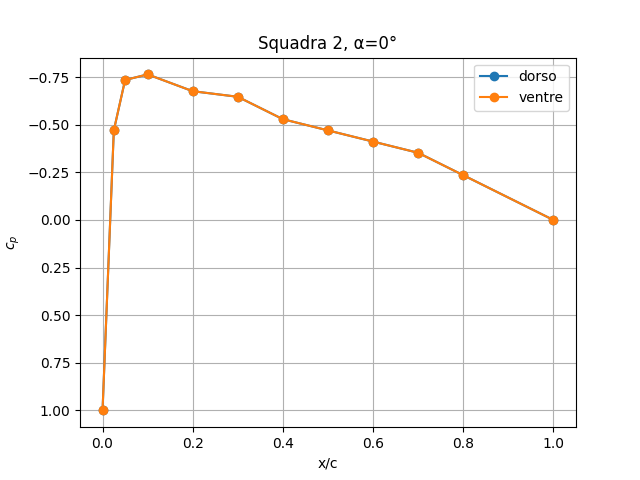
\includegraphics[width=.49\textwidth]{images/5/cp2 a=0.png}
    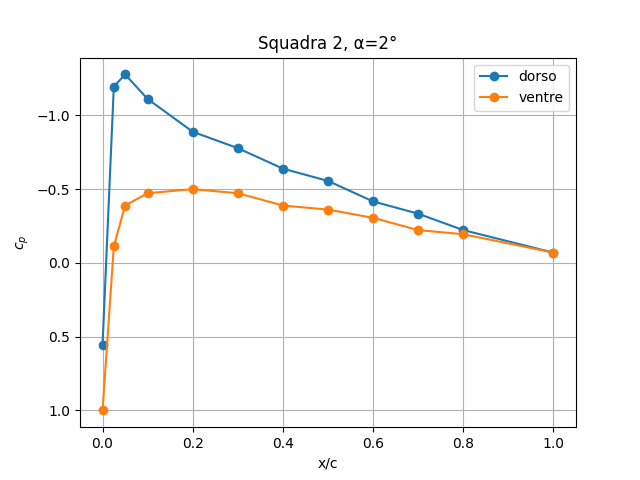
\includegraphics[width=.49\textwidth]{images/5/cp2 a=2.png}
    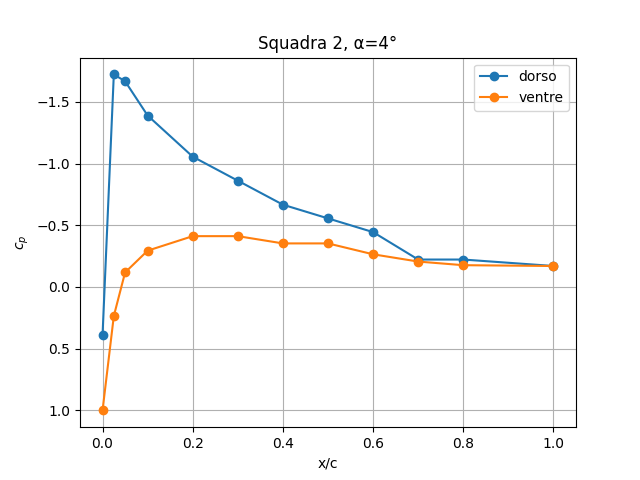
\includegraphics[width=.49\textwidth]{images/5/cp2 a=4.png}
    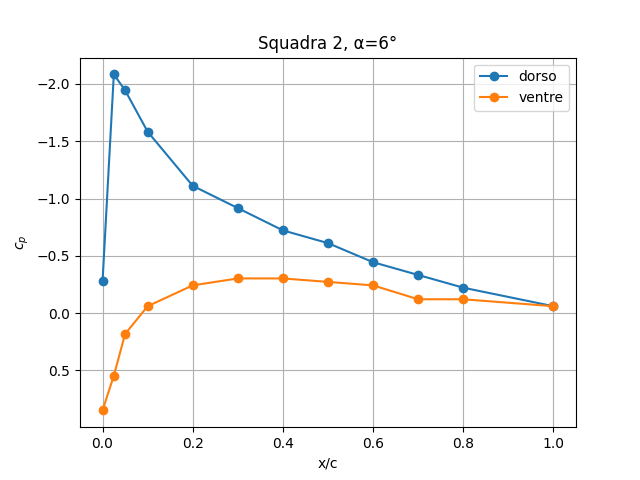
\includegraphics[width=.49\textwidth]{images/5/cp2 a=6.png}
    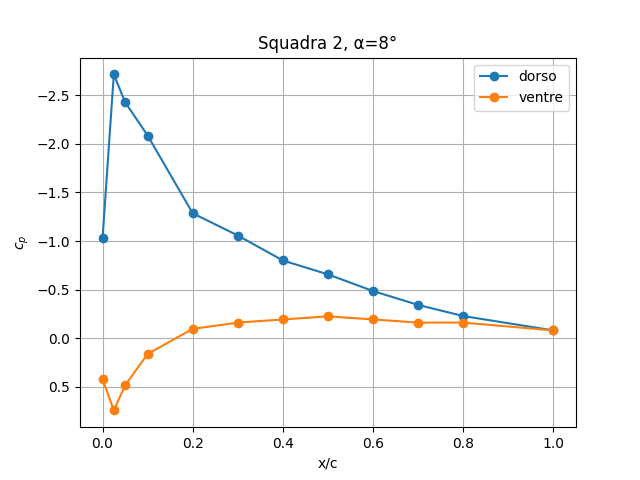
\includegraphics[width=.49\textwidth]{images/5/cp2 a=8.png}
    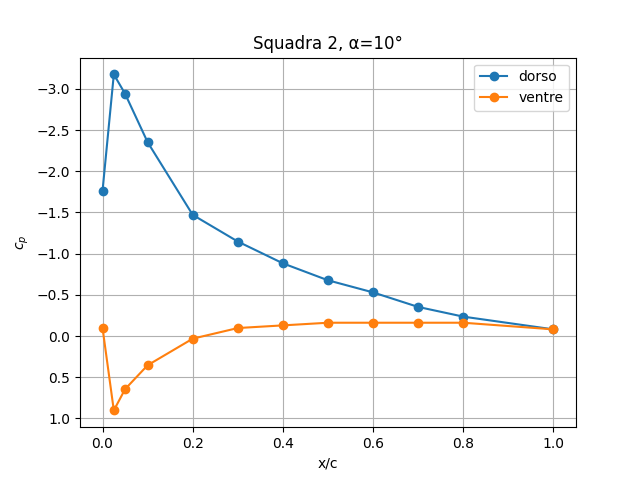
\includegraphics[width=.49\textwidth]{images/5/cp2 a=10.png}
    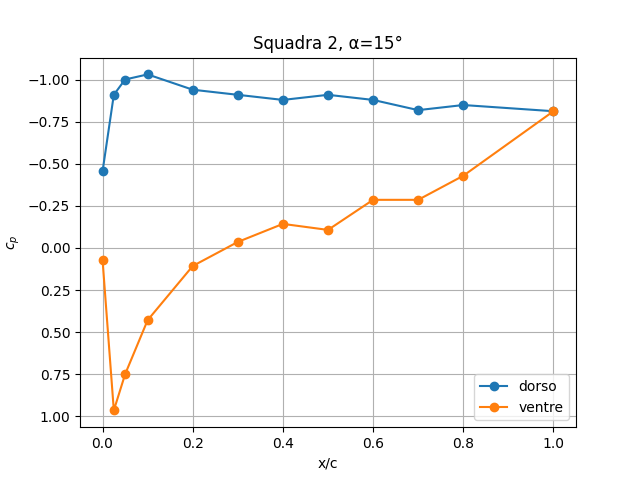
\includegraphics[width=.49\textwidth]{images/5/cp2 a=15.png}
    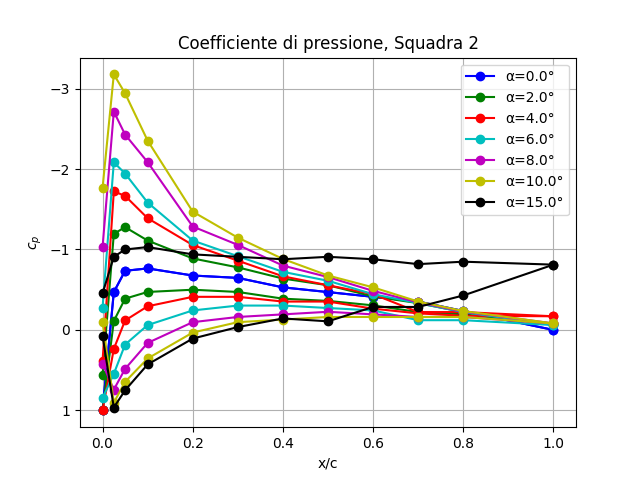
\includegraphics[width=.49\textwidth]{images/5/cp2.png}
\end{figure}
\begin{figure}[H]
    \centering
    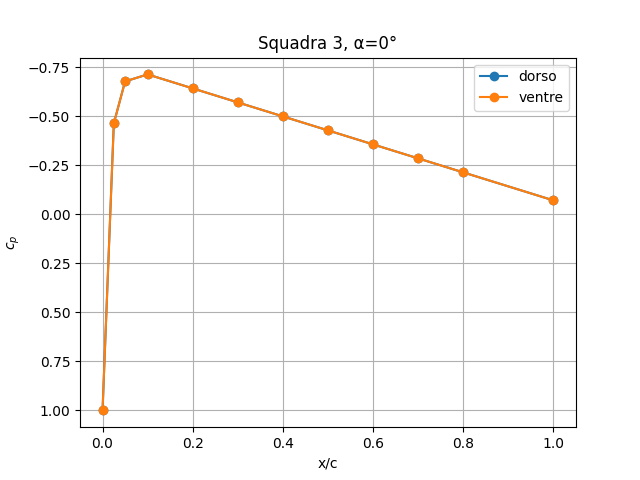
\includegraphics[width=.49\textwidth]{images/5/cp3 a=0.png}
    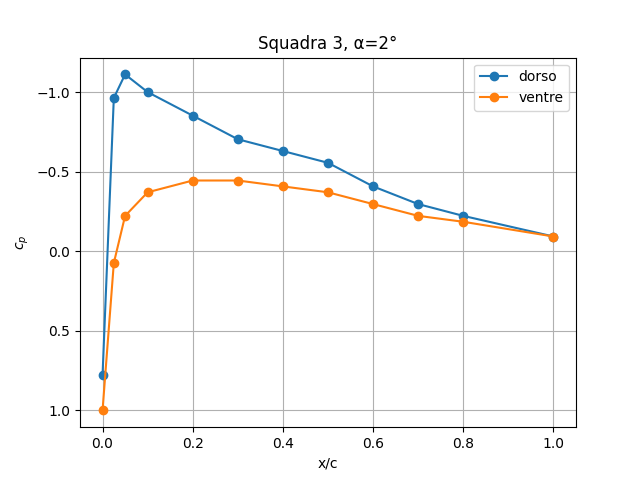
\includegraphics[width=.49\textwidth]{images/5/cp3 a=2.png}
    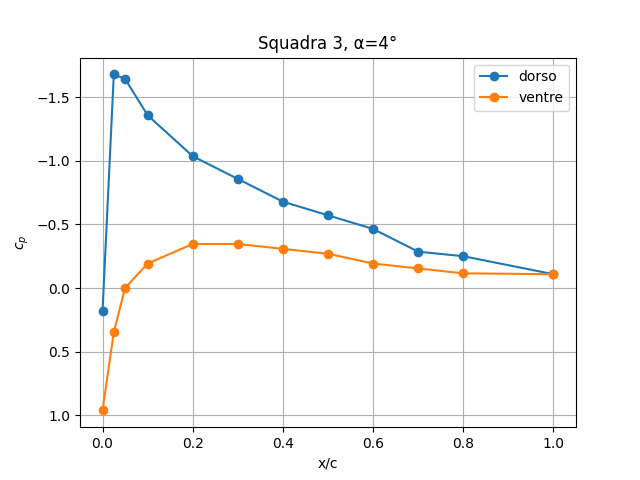
\includegraphics[width=.49\textwidth]{images/5/cp3 a=4.png}
    \includegraphics[width=.49\textwidth]{images/5/cp3 a=6.png}
    \includegraphics[width=.49\textwidth]{images/5/cp3 a=8.png}
    \includegraphics[width=.49\textwidth]{images/5/cp3 a=10.png}
    \includegraphics[width=.49\textwidth]{images/5/cp3 a=14.png}
    \includegraphics[width=.49\textwidth]{images/5/cp3.png}
\end{figure}
\begin{figure}[H]
    \centering
    \includegraphics[width=.49\textwidth]{images/5/cp4 a=0.png}
    \includegraphics[width=.49\textwidth]{images/5/cp4 a=2.png}
    \includegraphics[width=.49\textwidth]{images/5/cp4 a=4.png}
    \includegraphics[width=.49\textwidth]{images/5/cp4 a=6.png}
    \includegraphics[width=.49\textwidth]{images/5/cp4 a=10.png}
    \includegraphics[width=.49\textwidth]{images/5/cp4 a=12.png}
    \includegraphics[width=.49\textwidth]{images/5/cp4 a=15.png}
    \includegraphics[width=.49\textwidth]{images/5/cp4.png}
\end{figure}

\noindent Si nota come, alla presa di pressione statica posizionata sul bordo di attacco del profilo, si hanno due valori di coefficiente di pressione diversi tra dorso e ventre. Questo non è possibile fisicamente, si attribuisce tale discrepanza all'accuratezza della misura dell'angolo di incidenza sul goniometro nella camera di prova oppure ad un posizionamento della presa di pressione statica non perfettamente coincidente con il bordo di attacco del profilo.\\\\
Risulta inoltre evidente dall'andamento del coefficiente di pressione sul dorso come ad elevate incidenze ($\alpha > 12^\circ$) si verifichi lo stallo, infatti l'area sottesa tra le due curve, rappresentativa della portanza, si riduce drasticamente.\\\\
Questo era in realtà già evidente dalla visualizzazione delle canne manometriche:
\begin{figure}[H]
    \centering
    \includegraphics[width=.49\textwidth]{images/5/dsq1a10.png}
    \includegraphics[width=.49\textwidth]{images/5/dsq1a14.png}
    \caption{Istogrammi per la squadra 1 ad incidenza 10 e 14 gradi}
\end{figure}

\subsubsection{Confronto con teoria del flusso potenziale}
I risultati ottenuti per il coefficiente di pressione ad incidenza nulla confermano i risultati teorici della teoria del flusso potenziale, seppur con delle differenze, dovute alla mancanza della viscosità nella teoria del flusso potenziale.
\begin{figure}[H]
    \centering
    \includegraphics[width=.55\textwidth]{images/5/cpfp.png}
    \caption{Confronto con la teoria del flusso potenziale}
\end{figure}

\newpage
\subsubsection{Coefficiente di portanza}
Nota la distribuzione del coefficiente di pressione è possibile valutare il coefficiente di portanza del profilo $c_L$ al variare dell'incidenza $\alpha$:
\begin{equation*}
    c_L(\alpha) = \frac{L}{\frac12 \rho V_\infty^2 c} = \int_0^1 (c_{p-}-c_{p+})d\left( \frac xc \right)
\end{equation*}  
Poiché sono noti i valori del coefficiente di pressione in punti discreti, tale integrale è approssimato numericamente con l'utilizzo della regola dei trapezi:
\begin{equation*}
    \int_a^b f(x)dx \approx \sum_{k=1}^n \frac{f(x_{k-1}) + f(x_k)}2 \Delta x_k \quad \text{con } \Delta x_k = x_k - x_{k-1}
\end{equation*}
Pertanto si ottiene:
\begin{equation*}
    c_L(\alpha) = \sum_{k=1}^{11} \frac{(c_{p-}-c_{p+})_{k-1}+(c_{p-}-c_{p+})_k}2 \Delta \left( \frac xc \right)_k
\end{equation*}
Valutando il coefficiente di portanza ad ogni incidenza misurata si ottiene il diagramma $c_L$-$\alpha$ per le quattro squadre:
\begin{figure}[H]
    \centering
    \includegraphics[width=.75\textwidth]{images/5/cl.png}
    \caption{Coefficiente di portanza $c_L$ in funzione dell'incidenza $\alpha$}
\end{figure}

\noindent Si riscontra l'effetto dovuto alla variazione del numero di Reynolds, per un Reynolds più basso lo stallo risulta infatti più brusco, mentre per un Reynolds più elevato lo staoo è più morbido ed avviene ad un valore di $c_L$ maggiore.\\\\
Con un'interpolazione lineare dei primi punti del diagramma si può inoltre ricavare il coefficiente angolare di portanza $c_{L\alpha}\approx5.2$.

\subsubsection{Coefficiente di momento rispetto al bordo di attacco}
Analogamente al coefficiente di portanza, nota la distribuzione del coefficiente di pressione è possibile valutare il coefficiente di momento rispetto al bordo di attacco $c_{M_{LE}}$ al variare dell'incidenza $\alpha$:
\begin{equation*}
    c_{M_{LE}}(\alpha) = \frac{M_{LE}}{\frac12 \rho V_\infty^2 c^2} = \int_0^1 (c_{p+}-c_{p-})\left( \frac xc \right) d \left( \frac xc \right)
\end{equation*}
Anche in questo caso si valuta l'integrale numericamente utilizzando la regola dei trapezi:
\begin{equation*}
    \int_a^b f(x)dx \approx \sum_{k=1}^n \frac{f(x_{k-1}) + f(x_k)}2 \Delta x_k \quad \text{con } \Delta x_k = x_k - x_{k-1}
\end{equation*}\\

\noindent Si ottiene quindi il diagramma $c_{M_{LE}}$-$\alpha$ per le quattro squadre:
\begin{figure}[H]
    \centering
    \includegraphics[width=.85\textwidth]{images/5/cmle.png}
    \caption{Coefficiente di momento rispetto al bordo di attacco}
\end{figure}

\noindent Analogamente al coefficiente angolare di portanza, con un'interpolazione lineare dei primi punti del diagramma si ricava il coefficiente angolare del momento rispetto al bordo di attacco $c_{M_{LE}\alpha} \approx -1.3$.

\newpage
\subsubsection{Centro di pressione}
Il centro di pressione di un profilo alare rappresenta il punto in cui la risultante delle forze aerodinamiche (portanza e resistenza) può essere considerata applicata.
\begin{figure}[H]
    \centering
    \includegraphics[width=.7\textwidth]{images/5/xcpimage.png}
\end{figure}

\noindent Il centro di pressione varia la sua posizione con l'incidenza poiché dipende dal coefficiente di portanza e dal coefficiente di momento al bordo d'attacco:
\begin{equation*}
    M_{LE} = -L\cdot x_{cp} \quad \rightarrow \quad \frac{x_{cp}}c = - \frac{c_{M_{LE}}}{c_L} = f(\alpha)
\end{equation*}
Valutando il centro di pressione utilizzando i valori di coefficiente di portanza e momento rispetto al bordo di attacco precedentemente ricavata si ottiene il seguente diagramma per le quattro squadre:
\begin{figure}[H]
    \centering
    \includegraphics[width=.7\textwidth]{images/5/xcp.png}
\end{figure}

\noindent Il centro di pressione risulta mantenersi quasi costante ed in prossimità del fuoco aerodinamico finché il profilo non arriva alla condizione di stallo.\\\\
Non è possibile valutare la posizione del centro di pressione nel caso di incidenza nulla, questo perché il profilo, essendo simmetrico, ad incidenza nulla non genera portanza, quindi la posizione del centro di pressione risulta indefinita.

\subsubsection{Centro aerodinamico}
Nel centro aerodinamico, o fuoco, i profili alari godono della proprietà focale, cioè il coefficiente di momento aerodinamico risulta costante al variare dell'incidenza.\\\\
Si scrive la seguente equazione per il momento aerodinamico:
\begin{equation*}
    M_{ac} = -L(x_{cp} - x_{ac}) = -Lx_{cp} + Lx_{ac} = M_{LE} + Lx_{ac}
\end{equation*}
Si ricava quindi, in termini adimensionali:
\begin{equation*}
    c_{M_{ac}} = c_{M_{LE}} + c_L \frac{x_{ac}}c
\end{equation*}
Per il calcolo della posizione del fuoco si impone la proprietà focale, avendo cura di sostituire l'espressione per il $c_{M_{LE}}=c_{M_{LE}\alpha}\cdot\alpha$ e per il $c_L=c_{L\alpha}\cdot\alpha$ nel tratto lineare delle rispettive curve. Si giunge quindi al seguente risultato:
\begin{equation*}
    \frac{x_{ac}}c = - \frac{c_{M_{LE}\alpha}}{c_{L\alpha}} = \frac{1.3}{5.2} = 0.25
\end{equation*}
Questo risultato è valido per il campo subsonico mentre in campo supersonico il fuoco dei profili alari è posizionato in corrispondenza del 50\% della corda.

\subsubsection{Coefficiente di momento aerodinamico}
Una volta calcolata la posizione del fuoco si può ricavare il coefficiente di momento aerodinamico:
\begin{equation*}
    c_M = c_{M_{LE}} + c_L \frac{x_{ac}}c
\end{equation*}
Si ottiene quindi il seguente diagramma per le quattro squadre, che risulta verificare la proprietà focale del profilo:
\begin{figure}[H]
    \centering
    \includegraphics[width=.65\textwidth]{images/5/cm.png}
    \caption {Coefficiente di momento aerodinamico}
\end{figure}